\documentclass [a4paper] {article}
\usepackage[utf8]{inputenc}
\title{PRÁCTICA 3 FUNDAMENTOS DE LA CIENCIA DE DATOS}
\author{Javier Martín Gómez, Ignacio Afuera Díaz, Laura Gil Gómez, & Christian Ayala Urbanos}
\usepackage{Sweave}
\begin{document}
\maketitle

\begin{abstract}
En esta práctica hemos realizado un análisis de clasificación de datos con R. Para los datos cualitativos,
hemos utilizado el algoritmo de Hunt, y hemos resuelto el mismo problema visto en teoría. Hemos obtenido
la ganancia de información a través de la medida de impureza Gini. Además, hemos realizado otro análisis 
para variables cuantitativas, el análisis de regresión lineal. Hemos realizado el análisis de regresión 
para el radio y la densidad de los planetas interiores. Posteriormente, hemos añadido modificaciones a ambos
ejercicios.

\end{abstract}

\newpage
\tableofcontents
\newpage


\section{Primera parte}

En esta primera parte se realizará, con ayuda del lenguaje R, los ejercicios que hemos visto en teoría.

\subsection{Análisis de clasificación de datos cualitativos}

Se va a realizar el ejercicio de clasificación de datos cualitativos sobre el fichero datos.txt, que está formado
por cuatro calificaciones de 9 estudiantes. Dichas calificaciones se subdividen a su vez en dos grupos: por una
parte se tienen tres calificaciones iniciales de teoría (T), laboratorio (L), prácticas (P), que pueden ser A,B,C
o D, y otra calificación llamada calificación global (CG) que puede ser Ap o Ss. Para ello, se van a clasificar en 
aprobados o suspensos utilizando árboles de decisión de HuntPara empezar tendremos que
instalar y cargar la librería rpart, que es el paquete que permite la implementación de los árboles de
clasificación a utilizar:

\begin{Schunk}
\begin{Sinput}
> install.packages("rpart")
> library(rpart)
\end{Sinput}
\end{Schunk}

A continuación, leemos los datos del fichero datos.txt y los insertamos en un dataframe:

\begin{Schunk}
\begin{Sinput}
> calificaciones<-read.table("datos.txt")
> muestra=data.frame(calificaciones)
> muestra
\end{Sinput}
\begin{Soutput}
  T L P CG
1 A A B Ap
2 A B D Ss
3 D D C Ss
4 D D A Ss
5 B C B Ss
6 C B B Ap
7 B B A Ap
8 C D C Ss
9 B A C Ss
\end{Soutput}
\end{Schunk}

Tras insertar los datos en el dataframe, los clasificamos utilizando rpart, donde CG es el suceso
clasificador (el punto de después de CG~ indica que para la función de clasificación se van a usar todos
las variables restantes de la muestra). Primero analizaremos el árbol de decisión con el algoritmo Gini:


\begin{Schunk}
\begin{Sinput}
> clasificacion=rpart(CG~.,data=muestra,method="class",minsplit=1)
\end{Sinput}
\end{Schunk}


Otra forma de realizar lo anterior es como sigue (aquí indicamos los elementos en vez de escribir un punto):

\begin{Schunk}
\begin{Sinput}
> clasificacion=rpart(CG~T+L+P, data=muestra, method="class", minsplit=1)
\end{Sinput}
\end{Schunk}

Vemos la estructura del árbol y observamos que realiza la clasificación:

\begin{Schunk}
\begin{Sinput}
> clasificacion
\end{Sinput}
\begin{Soutput}
n= 9 

node), split, n, loss, yval, (yprob)
      * denotes terminal node

1) root 9 3 Ss (0.3333333 0.6666667)  
  2) L=A,B 5 2 Ap (0.6000000 0.4000000)  
    4) P=A,B 3 0 Ap (1.0000000 0.0000000) *
    5) P=C,D 2 0 Ss (0.0000000 1.0000000) *
  3) L=C,D 4 0 Ss (0.0000000 1.0000000) *
\end{Soutput}
\end{Schunk}

Ahora se analizará el árbol mediante entropía:

\begin{Schunk}
\begin{Sinput}
> clasificacion2=rpart(CG~., data=muestra,method="class",
+ minsplit=1,parms=list(split="information"))
\end{Sinput}
\end{Schunk}

De nuevo, visualizamos la estructura del árbol mediante el nuevo algoritmo:

\begin{Schunk}
\begin{Sinput}
> clasificacion2
\end{Sinput}
\begin{Soutput}
n= 9 

node), split, n, loss, yval, (yprob)
      * denotes terminal node

1) root 9 3 Ss (0.3333333 0.6666667)  
  2) L=A,B 5 2 Ap (0.6000000 0.4000000)  
    4) P=A,B 3 0 Ap (1.0000000 0.0000000) *
    5) P=C,D 2 0 Ss (0.0000000 1.0000000) *
  3) L=C,D 4 0 Ss (0.0000000 1.0000000) *
\end{Soutput}
\end{Schunk}

\subsection{Análisis de clasificación de datos cuantitativos}

Vamos a realizar un análisis de regresión para el fichero datos2.txt, que muestra los radios ecuatoriales
(R) y densidades (D) de los planetas interiores del sistema solar (ya que a diferencia del apartado anterior
estos datos son numéricos, y por tanto, cuantitativos). Para ello, leemos los datos del archivo correspondiente:

\begin{Schunk}
\begin{Sinput}
> muestra2=read.table("datos2.txt")
> muestra2
\end{Sinput}
\begin{Soutput}
           R   D
Mercurio 2.4 5.4
Venus    6.1 5.2
Tierra   6.4 5.5
Marte    3.4 3.9
\end{Soutput}
\end{Schunk}

Para realizar el análisis de regresión utilizamos lm, ya que es la función de R que ajusta modelos lineales,
y en ella especificamos la relación deseada. En nuestro caso será D y R:

\begin{Schunk}
\begin{Sinput}
> regresion=lm(D~R,data=muestra2)
> regresion
\end{Sinput}
\begin{Soutput}
Call:
lm(formula = D ~ R, data = muestra2)

Coefficients:
(Intercept)            R  
     4.3624       0.1394  
\end{Soutput}
\end{Schunk}

También, podemos ver un resumen del análisis de regresión en el que se muestran datos interesantes sobre la recta,
como los residuos, los coeficientes, el error residual estándar y la correlación cuadrada. Para ello hacemos uso
de la función summary: 

\begin{Schunk}
\begin{Sinput}
> summary(regresion)
\end{Sinput}
\begin{Soutput}
Call:
lm(formula = D ~ R, data = muestra2)

Residuals:
Mercurio    Venus   Tierra    Marte 
 0.70312 -0.01253  0.24566 -0.93624 

Coefficients:
            Estimate Std. Error t value Pr(>|t|)  
(Intercept)   4.3624     1.2050   3.620   0.0685 .
R             0.1394     0.2466   0.565   0.6289  
---
Signif. codes:  0 ‘***’ 0.001 ‘**’ 0.01 ‘*’ 0.05 ‘.’ 0.1 ‘ ’ 1

Residual standard error: 0.846 on 2 degrees of freedom
Multiple R-squared:  0.1377,	Adjusted R-squared:  -0.2935 
F-statistic: 0.3193 on 1 and 2 DF,  p-value: 0.6289
\end{Soutput}
\end{Schunk}


\section{Segunda parte}

En esta sección detallaremos las mejoras que hemos realizado sobre los ejercicios de la sección anterior.

\subsection{Mejoras en la clasificación de datos cualitativos}
Para esta sección ha sido necesario recurrir, a parte de rpart, a los paquetes y librerias plotmo y rpart.plot para
poder visualizar los árboles de decisión de forma más clara. Para ello se realiza su correspondiente instalación:

\begin{Schunk}
\begin{Sinput}
> install.packages("rpart")
> install.packages("rpart.plot")
> install.packages("plotmo")
> library(rpart)
> library(rpart.plot)
> library(plotmo)
\end{Sinput}
\end{Schunk}

La primera mejora para este ejercicio consiste en poder visualizar de forma gráfica el árbol de decisión.
Para ello se utiliza la siguiente instrucción, donde type=5 sirve para poder ver en cada nodo el nombre
de su correspondiente variable.

\begin{Schunk}
\begin{Sinput}
> rpart.plot(clasificacion,type=5)
\end{Sinput}
\end{Schunk}
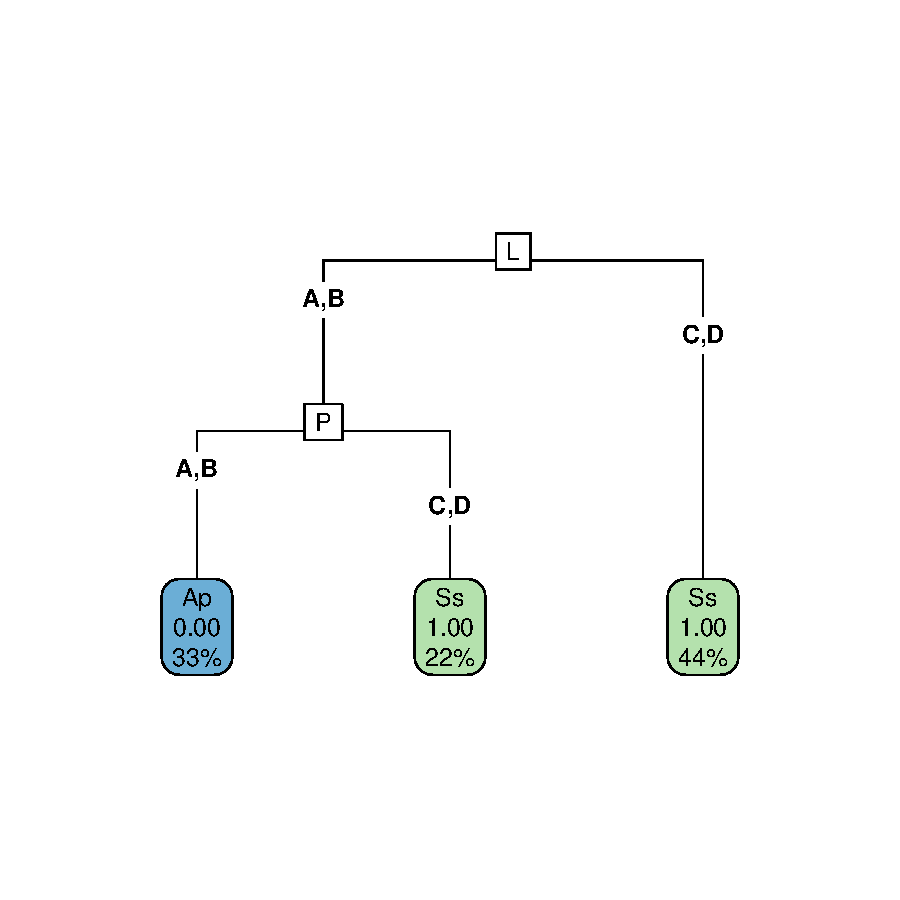
\includegraphics{Memoria-Figura 1}

\newpage
Hacemos lo mismo con el árbol de decisión analizado con entropía:

\begin{Schunk}
\begin{Sinput}
> rpart.plot(clasificacion2,type=5)
\end{Sinput}
\end{Schunk}
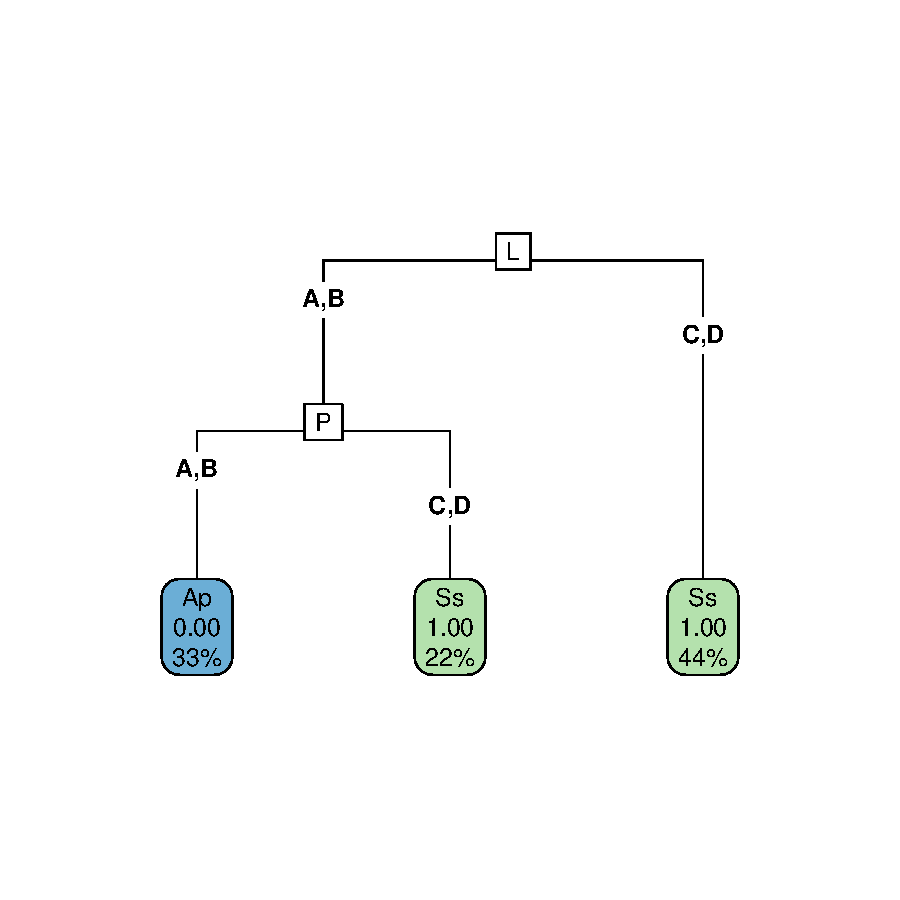
\includegraphics{Memoria-Figura 2}

\newpage
Otro tipo de árbol que podemos visualizar es el que se muestra a continuación, este nos muestra, a parte
de las decisiones tomadas en cada rama, la cantidad de datos de cada tipo (en nuestro caso Ap y Ss)
que cada nodo posee.

\begin{Schunk}
\begin{Sinput}
> plot(clasificacion, uniform=TRUE, 
+ main="Arbol de clasificacion para las asignaturas")
> text(clasificacion, use.n=TRUE, all=TRUE, 
+ cex=.7, fancy=TRUE, fwidth=0.5, fheight=0.7)
\end{Sinput}
\end{Schunk}
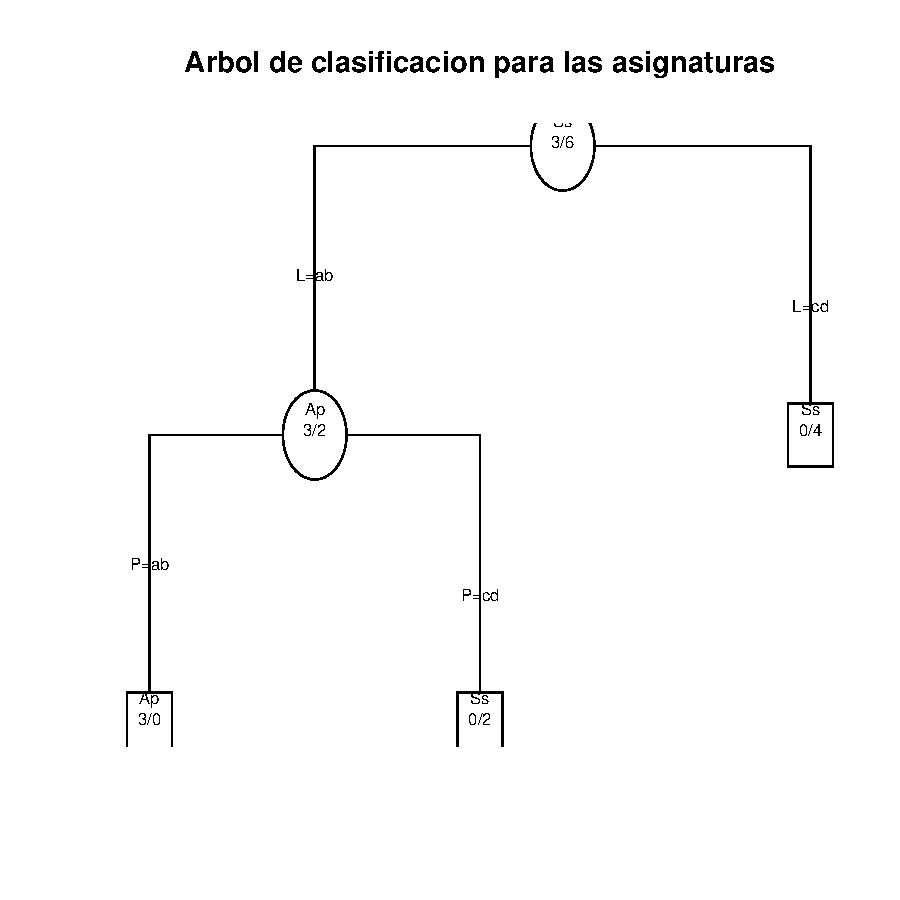
\includegraphics{Memoria-Figura 3}

\newpage
Lo mismo para entropía:

\begin{Schunk}
\begin{Sinput}
> plot(clasificacion2, uniform=TRUE, 
+ main="Arbol de clasificacion para las asignaturas mediante entropía")
> text(clasificacion2, use.n=TRUE, all=TRUE, 
+ cex=.7, fancy=TRUE, fwidth=0.5, fheight=0.7)
\end{Sinput}
\end{Schunk}
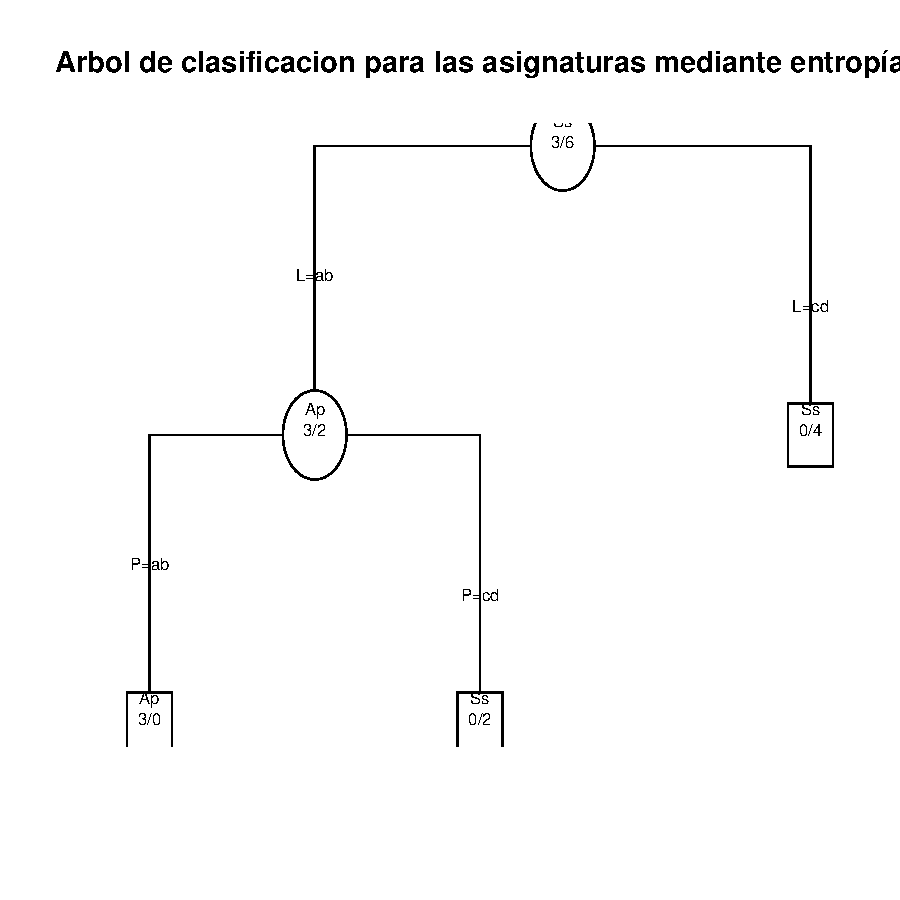
\includegraphics{Memoria-Figura 4}

La segunda mejora consiste en mostrar en texto las reglas de clasificación obtenidas para poder entenderlas
más facilmente. Para ello utiliza la instrucción rules:

\begin{Schunk}
\begin{Sinput}
> rpart.rules(clasificacion)
\end{Sinput}
\begin{Soutput}
   CG                               
 0.00 when L is A or B & P is A or B
 1.00 when L is A or B & P is C or D
 1.00 when L is C or D              
\end{Soutput}
\end{Schunk}

\newpage
Realizamos lo mismo con la entropía
\begin{Schunk}
\begin{Sinput}
> rpart.rules(clasificacion2)
\end{Sinput}
\begin{Soutput}
   CG                               
 0.00 when L is A or B & P is A or B
 1.00 when L is A or B & P is C or D
 1.00 when L is C or D              
\end{Soutput}
\end{Schunk}

\newpage
Para mostrar las reglas en formato gráfico se hace uso de prp, que muestra un modelo de tipo rpart:

\begin{Schunk}
\begin{Sinput}
> prp(clasificacion, extra = 7)
\end{Sinput}
\end{Schunk}
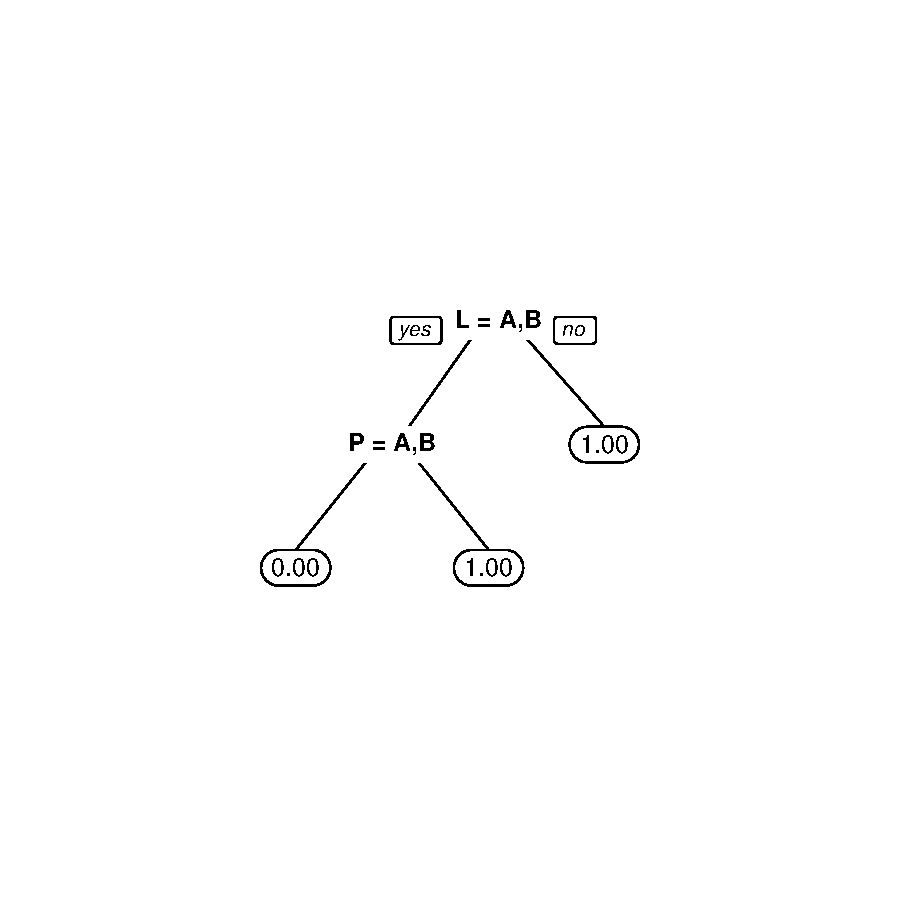
\includegraphics{Memoria-Figura 5}

\newpage
\begin{Schunk}
\begin{Sinput}
> prp(clasificacion2, extra = 7)
\end{Sinput}
\end{Schunk}
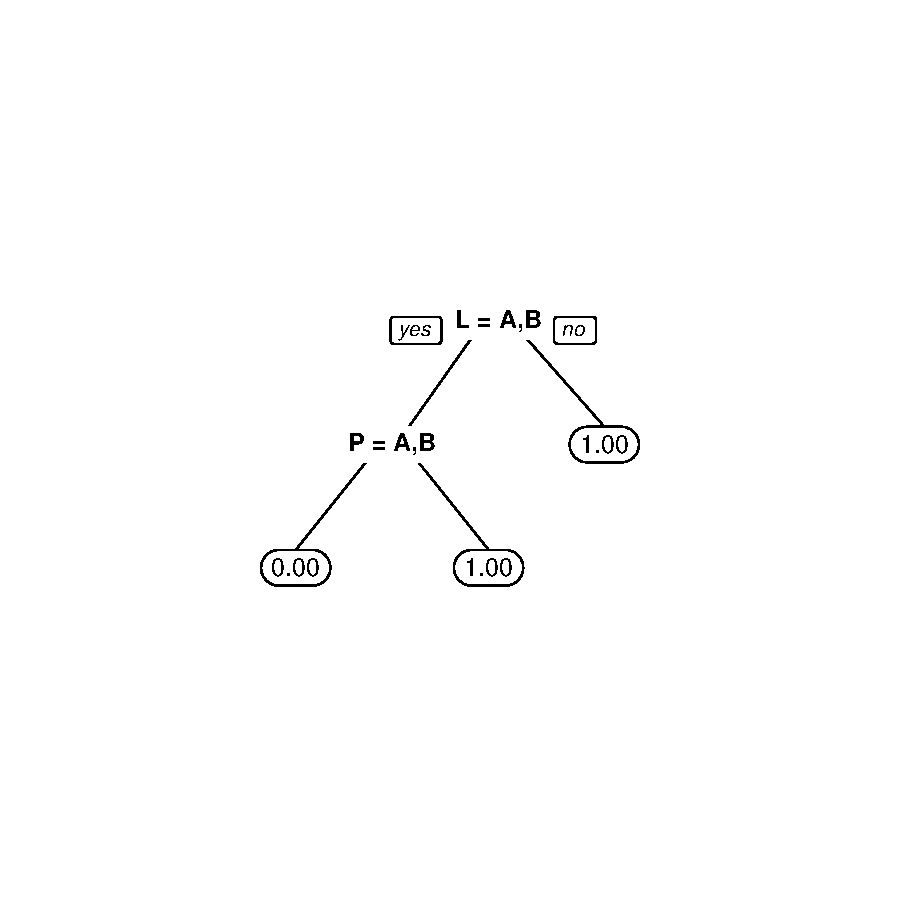
\includegraphics{Memoria-Figura 6}

Como última modificación a este apartado, se presentan unos gráficos en relación a las variables L y P
para el resultado final CG=Ap (tres primeros gráficos) y para el resultado final CG=Ss (tres últimos).

\begin{Schunk}
\begin{Sinput}
> plotmo(clasificacion, type = "prob", nresponse = "Ap")
\end{Sinput}
\begin{Soutput}
 plotmo grid:    T L P
                 B B B
\end{Soutput}
\begin{Sinput}
> plotmo(clasificacion, type = "prob", nresponse = "Ap",
+ type2 = "image", ngrid2 = 200,
+ pt.col = ifelse(kyphosis$Kyphosis == "Ap", "red", "lightblue"))
\end{Sinput}
\begin{Soutput}
 plotmo grid:    T L P
                 B B B
\end{Soutput}
\begin{Sinput}
> 
\end{Sinput}
\end{Schunk}
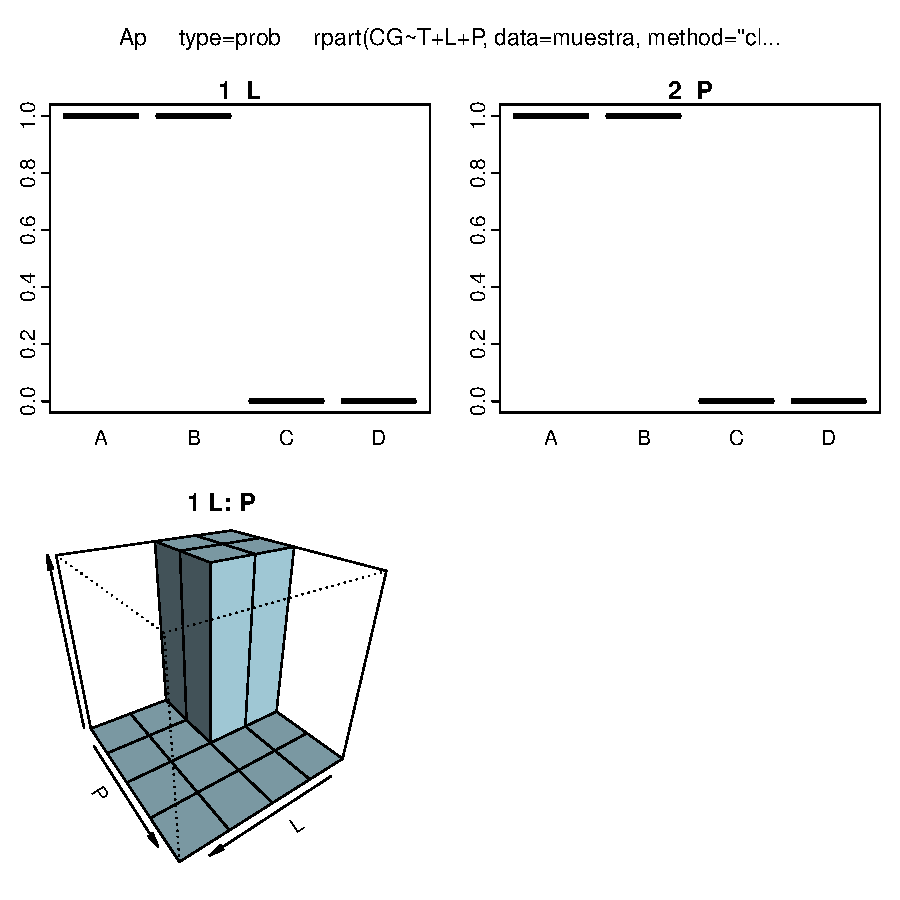
\includegraphics{Memoria-Figura 7}


\begin{Schunk}
\begin{Sinput}
> plotmo(clasificacion, type = "prob", nresponse = "Ss") # middle graph
\end{Sinput}
\begin{Soutput}
 plotmo grid:    T L P
                 B B B
\end{Soutput}
\begin{Sinput}
> plotmo(clasificacion, type = "prob", nresponse = "Ss",
+ type2 = "image", ngrid2 = 200,
+ pt.col = ifelse(kyphosis$Kyphosis == "Ss", "red", "lightblue"))
\end{Sinput}
\begin{Soutput}
 plotmo grid:    T L P
                 B B B
\end{Soutput}
\end{Schunk}
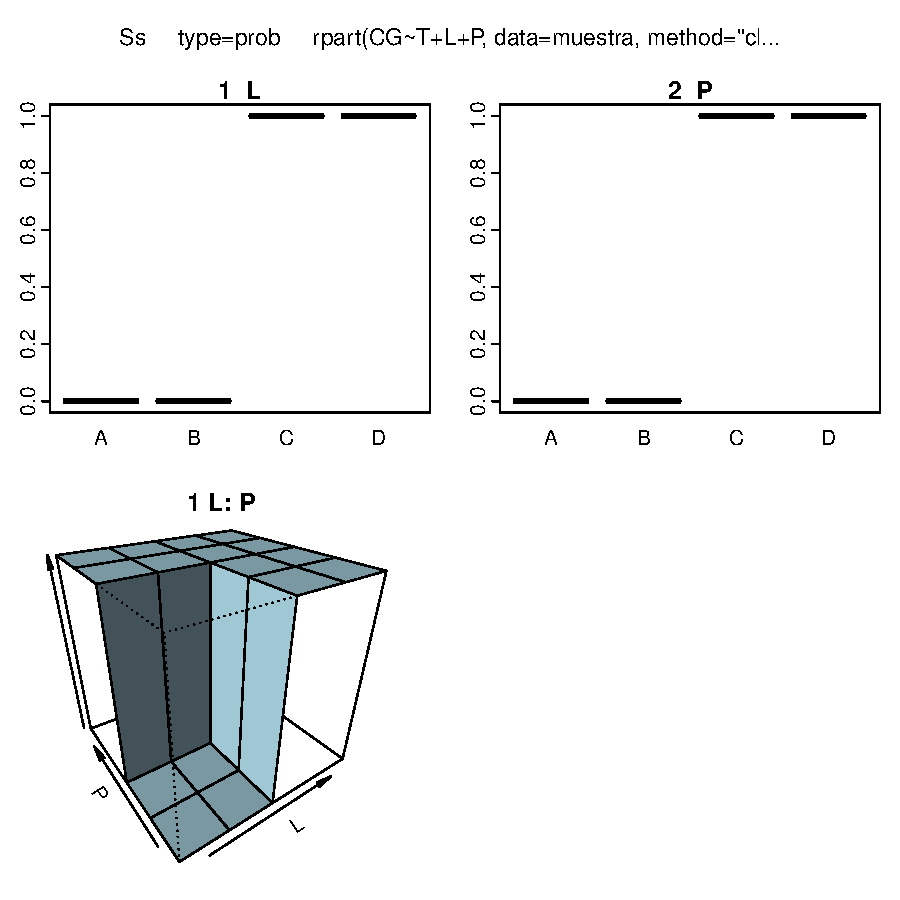
\includegraphics{Memoria-Figura 8}

Visualizamos los mismos gráficos para la entropía

\begin{Schunk}
\begin{Sinput}
> plotmo(clasificacion2, type = "prob", nresponse = "Ap") # middle graph
\end{Sinput}
\begin{Soutput}
 plotmo grid:    T L P
                 B B B
\end{Soutput}
\begin{Sinput}
> plotmo(clasificacion2, type = "prob", nresponse = "Ap",
+ type2 = "image", ngrid2 = 200,
+ pt.col = ifelse(kyphosis$Kyphosis == "Ap", "red", "lightblue"))
\end{Sinput}
\begin{Soutput}
 plotmo grid:    T L P
                 B B B
\end{Soutput}
\end{Schunk}
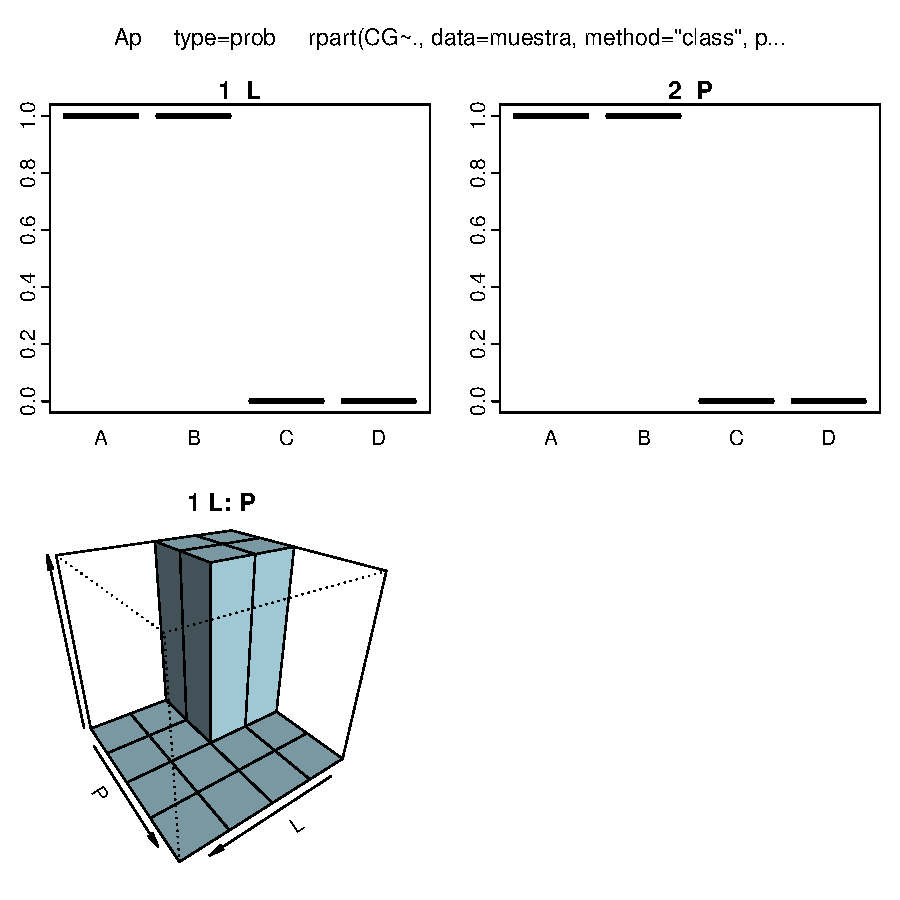
\includegraphics{Memoria-Figura 9}

\begin{Schunk}
\begin{Sinput}
> plotmo(clasificacion2, type = "prob", nresponse = "Ss") # middle graph
\end{Sinput}
\begin{Soutput}
 plotmo grid:    T L P
                 B B B
\end{Soutput}
\begin{Sinput}
> plotmo(clasificacion2, type = "prob", nresponse = "Ss",
+ type2 = "image", ngrid2 = 200,
+ pt.col = ifelse(kyphosis$Kyphosis == "Ss", "red", "lightblue"))
\end{Sinput}
\begin{Soutput}
 plotmo grid:    T L P
                 B B B
\end{Soutput}
\end{Schunk}
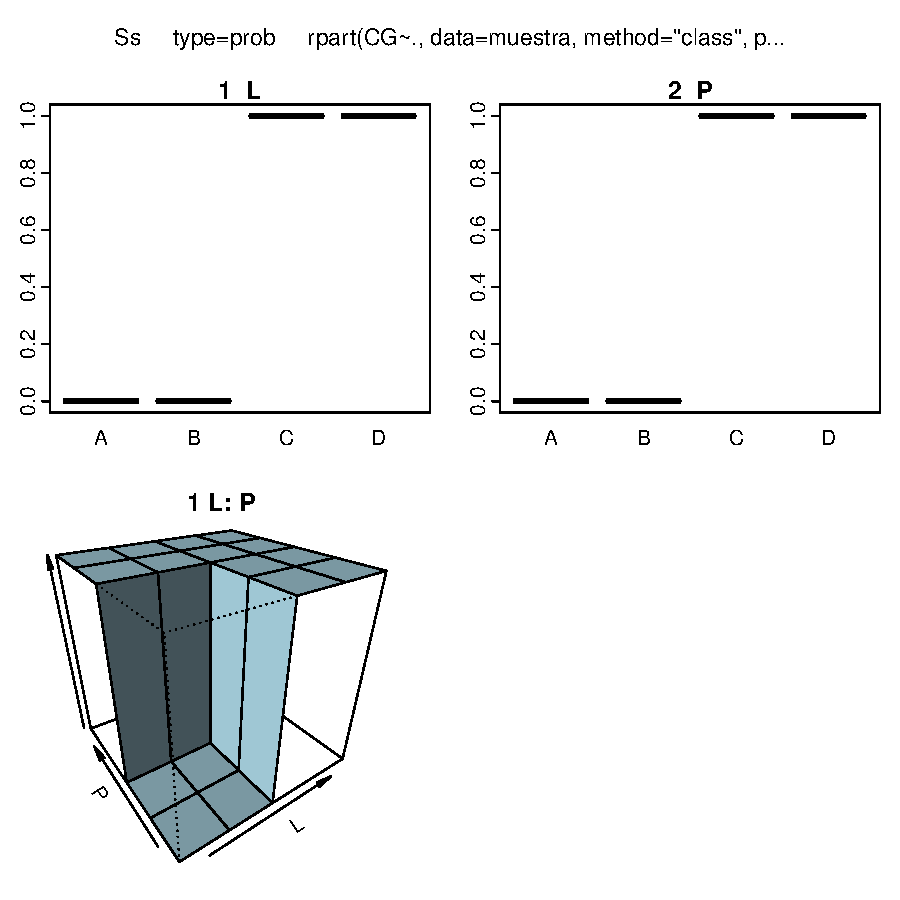
\includegraphics{Memoria-Figura 10}


\newpage
\subsection{Mejoras en la clasificación de datos cuantitativos}
Aquí representaremos la recta que hemos obtenido en el proceso de la regresión, además de las muestras:

\begin{Schunk}
\begin{Sinput}
> plot(muestra2$R, muestra2$D, xlab='Radio', ylab='Densidad')
> abline(regresion,col="red")
> predict(regresion, muestra2) #Segunda variable
\end{Sinput}
\begin{Soutput}
Mercurio    Venus   Tierra    Marte 
4.696877 5.212535 5.254345 4.836244 
\end{Soutput}
\end{Schunk}
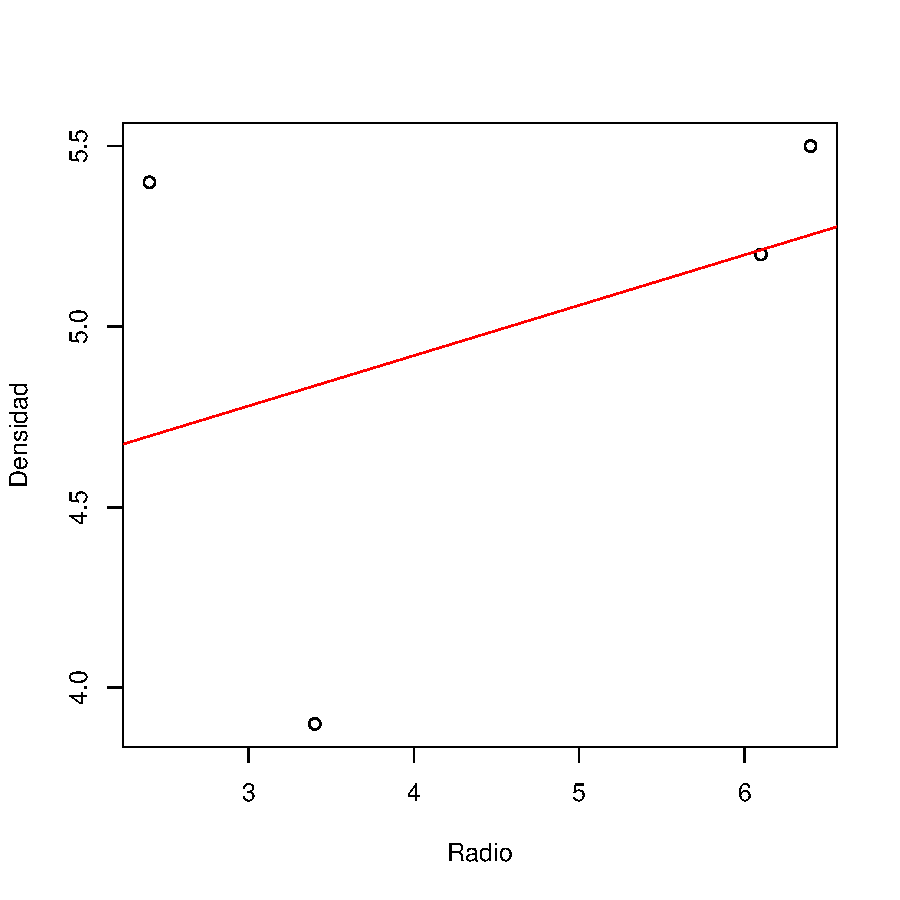
\includegraphics{Memoria-Figura 11}

\subsubsection{Creación de funciones para el análisis de regresión}

En esta subsección vamos a crear las funciones vistas en teoría para el análisis de regresión.

En primer lugar se ha creado una función que calcula la covarianza siguiendo exactamente el mismo procedimiento
que hemos visto en teoría

\begin{Schunk}
\begin{Sinput}
> covarianza<-function(x,y) {
+ 	media_x<-mean(x)
+ 	media_y<-mean(y)
+ 	len<- length(x)
+ 	res<-0
+ 	for(i in 1:len){
+ 		res<-res+x[i]*y[i]
+ 	}
+ 	res/len-media_x*media_y
+ }
> covarianza(radio,densidad)
\end{Sinput}
\begin{Soutput}
[1] 0.41
\end{Soutput}
\end{Schunk}

Ahora, usaremos la covarianza para el cálculo de la función de regresión y la correlación, que nos indicará
cuánta dependencia habrá entre las variables (cuanto más cerca de 1 -,1 mejor y más cerca de 0, peor).
Para ello, primero tendremos que crear la fórmula de la desviación típica (creada en la práctica 1):

\begin{Schunk}
\begin{Sinput}
> sd_nuestra=function(x){sqrt((sd(x)^2)*(length(x)-1)/length(x))}
\end{Sinput}
\end{Schunk}

Con la covarianza y las desviaciones típicas de las dos variables. Obtenemos la correlación:


\begin{Schunk}
\begin{Sinput}
> correlacion<-function(x,y){covarianza(x,y)/(sd_nuestra(x)*sd_nuestra(y))}
> correlacion(densidad,radio)
\end{Sinput}
\begin{Soutput}
[1] 0.371063
\end{Soutput}
\end{Schunk}

Para calcular la función de regresión (y=a+bx), tendremos que hallar primero los valores de a y b, los cuales
se obtendrán a partir de las funciones creadas anteriormente:

\begin{Schunk}
\begin{Sinput}
> b_recta<-function(x,y){covarianza(x,y)/(sd_nuestra(x) * sd_nuestra(x))}
> a_recta<-function(x,y){
+ 	b<-b_recta(x,y)
+ 	mean(y)-mean(x)*b
+ }
\end{Sinput}
\end{Schunk}

Ahora, a partir de los valores a y b calculados anteriormente, se construye la recta con la siguiente función:

\begin{Schunk}
\begin{Sinput}
> recta<-function(x,y){
+ 	b<-b_recta(x,y)
+ 	a<-a_recta(x,y)
+ 	r<-correlacion(x,y)
+ 	paste("y =",as.character(a),"+",as.character(b),"* x",sep=" ")
+ 	
+ }
> recta(radio,densidad)
\end{Sinput}
\begin{Soutput}
[1] "y = 4.36239643084767 + 0.139366900361164 * x"
\end{Soutput}
\end{Schunk}


Tambien se ha implementado el análisis ANOVA para las rectas de regresión. Para ello se han creado las siguientes funciones:

-SSR: calcula según el procedimiento visto en teoría el dato con el mismo nombre (el sumatorio cada valor de y calculado menos la media 
al cuadrado, es decir, se calcula cuanto se alejan los valores calculados de y de la media):

\begin{Schunk}
\begin{Sinput}
> SSR<-function(x,y){
+ 	media_y<-mean(y)
+ 	a<-a_recta(x,y)
+ 	b<-b_recta(x,y)
+ 	len<- length(x)
+ 	res<-0
+ 	for(i in 1:len){
+ 		y_aux<-a+b*x[i]
+ 		res<-res+(y_aux-media_y)*(y_aux-media_y)
+ 	}
+ 	res
+ }
\end{Sinput}
\end{Schunk}

-SSY: calcula el sumatorio de cada valor de y observado menos la media al cuadrado, en otras palabras, calculamos cuanto se alejan los valores
observados de y de la media:

\begin{Schunk}
\begin{Sinput}
> SSY<-function(x,y){
+ 	media_y<-mean(y)
+ 	len<-length(x)
+ 	res<-0
+ 	for(i in 1:len){
+ 		res<-res+(y[i]-media_y)*(y[i]-media_y)
+ 	}
+ 	res
+ }
\end{Sinput}
\end{Schunk}

-Correlación cuadrada: haciendo el cociente de los dos valores anteriores (SSR/SSY) obtendremos un dato cuyo valor
esta comprendido entre 0 y 1, contra más cerca de 1 este mejor ajustada estará la recta.

\begin{Schunk}
\begin{Sinput}
> correlacion_cuadrada<-function(x,y){SSR(x,y)/SSY(x,y)}
> correlacion_cuadrada(radio,densidad)
\end{Sinput}
\begin{Soutput}
[1] 0.1376878
\end{Soutput}
\end{Schunk}

Tambien se ha implementado el error estándar de la estimación, que es la diferencia entre los valores de y
a través de la función de regresión. Cuanto más próximo a 0 sea, nos indicará un buen ajuste de la recta :

\begin{Schunk}
\begin{Sinput}
> sr<-function(x,y){
+ 	a<-a_recta(x,y)
+ 	b<-b_recta(x,y)
+ 	len<- length(x)
+ 	res<-0
+ 	for(i in 1:len){
+ 		y_aux<-a+b*x[i]
+ 		res<-res+(y_aux-y[i])*(y_aux-y[i])
+ 	}
+ 	sqrt(res/len)
+ }
> sr(radio,densidad)
\end{Sinput}
\begin{Soutput}
[1] 0.5982136
\end{Soutput}
\end{Schunk}

\section{Conclusiones}
En esta práctica hemos aprendido a como realizar la clasificación supervisada con ayuda del lenguaje de programación R.
En concreto a como realizar el algoritmo de Hunt y a realizar un análisis de regresión. Tambien hemos aprendido a poder
representar los datos que se obtienen de dichos análisis para poderlos visualizar de una forma más sencilla. Por último,
nosotros también hemos creado parte de dichos análisis como puede ser el ANOVA u otras medidas del ajuste de la recta de
regresión.















\end{document}
